\chapter{Análisis de intervalos}

El Análisis de Intervalos es una rama de las Matemáticas que lidia con los proclemas de redondeo debido al uso de la aritmética de coma flotante. Los ordenadores tienen registros de coma flotante para representar los números reales. Como es bien sabido, hay número reales que no tienen representación finita, por esa razón estos nñumeros tienen que ser redondeados.
\par Este tipo de situación crea problemas de imprecisión numérica que se puede propagar y acumular a los largo de los algoritmos, en especial en aquellos que son recursivos.
\par Aunque es posible trabajar con un gran tamaño de bits para representar a los números, este conjunto de números es, de hecho, una representación digital que, obviamente, no tiene las mismas propiedades que el conjunto de números reales.
\par Un ejemplo muy básico puede mostarnos este problema:
\begin{itemize}
	\item a = \texttt{random()}
	\item b = \texttt{random()}
	\item c = a + b
	\item c = c - a - b
\end{itemize}
Por lógica de como trabajamos con el conjunto de números reales se esperaría que el valor final de $c$ sea cero, pero este puede no ser el caso dependiendo del programa de cálculo que tomemos en un ordenador convencional.
\par Hay una gran cantidad de áreas de investigación en las cuales en Análisis de Intervalos ha sido aplicado para mantener la precisión numérica: Ingeniería de control y supervisión, modelización geométrica y diseño por ordenador.
\par Aparte también hay una serie de{ \em catástrofes} documentadas que podrían haber sido evitadas usando Análisis de Intervalos. Por ejemplo:
\begin{itemize}
	\item Un misil Patriot falló debido a la acumulación de errores de redondeo.
	\item La explosión del Arianne 5 causada por un error de exceso.
\end{itemize}
En este capítulo presentaremos la nociones, operaciones y propiedades básicas del Análisis de Intervalos. Además también haremos una introducción al Análisis de intervalos Modal que completa la definición clásica de Análisis de Intervalos.

\section{Planteamiento}

La computación numérica de problemas teóricos en un ordenador requiere que los número sreales $\mathbb{R}$ sean representados con una cantidad limitada de cifras decimales. Por supuesto, es posible usar un conjunto de números suficientemente grande de números con una gran cantidad de cifras decimales, pero aún así habrá números reales que no podrán ser representados.
\par Esto significa que, cuando traducimos un problema teórico a un problema computacional, estamos trabajando con un conjunto de{ \em números digitales}, llámese DI, también conocidos como números en coma flotante.
\par Los números reales dan soporte a aquellos modelos donde las magnitudes continuas están presentaes. Sin embargo, como sabemos, los ordenadores trabajan con truncamiento de números reales. Por tanto, es posible que parate de la información se pierda. Las operaciones deberían restringirse a un intervalo obtenido por medias de redondeo, lo que nos da una identificaciñon operacional de los valores calculados.
\par Dados dos valores reales $\underline{a}$ y $\overline{a}$, un intervalo $A$ se define como:

\begin{equation}
A = [\underline{a},\overline{a}] = \{ x \in \mathbb{R} : \underline{a} \leq x \leq \overline{a} \}
\nonumber
\end{equation}

en donde $\underline{a}$ y $\overline{a}$ se conocen como el ínfimo y el supremo del intervalo respectivamente.
\par FRASE QUE NECESITO REVISAR. El uso del Análisis de Intervalos con números digitales nos proporciona un control automático de los errores de redondeo.
\par En la construcción de intervalos, denotados por $I(\mathbb{R})$, muchas de las propiedades de los números reales se pierden, véase la propiedad distributiva, y se obtienen otras como la relación de inclusión.
\par Los ordenadores trabajan con el conjunto $DI$, por esa razón el conjunto de intervalos con base en $DI$, denotado por $I(DI)$, es el usado para las operaciones algorítmicas. Esto significa que, mientras $I(DI)$ admita operaciones sobre el conjunto $DI$ para ser tratadas por ordenador, se puede establecer un modelo analítico de operaciones y relaciones de los intervalos análogo al de los intervalos $I(\mathbb{R})$.
\par Como los intervalos que trataremos a a partir de ahora no son intervalos de números reales significa que los algoritmos que aplicamos a éstos deberán ser modificados para adaptarse a la nueva aritmética.

\section{Relaciones entre intervalos}

Las relaciones entre los intervalos son equivalentes a algunas relaciones entre los límites del intervalo. Aunque la definición de las relaciones a veces no son evidentes, hay una norma general de tomar la definición más útil en cada caso. Lo importante esobtener relaciones parecidas a los intervalos de números reales.

\begin{definition}
Se dice que dos intervalos $A$ y $B$ son iguales, denotado por $A = B$, si para todo $a \in A$ exite $b \in B$ tal que $a = b$ y viceversa. En función de los límites:

$$A = B \iff \underline{a} = \underline{b} \text{ y } \overline{a} = \overline{b}$$
\end{definition}

\begin{definition}
Se dice que dados dos intervalos, $A$ y $B$, $A < B$ si para todo $a \in A$ y $b \in B$ se tiene que $a < b$. En función de los límites:

$$A < B \iff \overline{a} < \underline{b}$$
\end{definition}

\begin{definition}
Se dice que dados dos intervalos, $A$ y $B$, $A \leq B$ si para todo $a \in A$ existe $b \in B$ tal que $a \leq b$ y para todo $b \in B$ existe $a \in A$ tal que $a \leq b$. En función de los límites:

$$A \leq B \iff \underline{a} \leq \underline{b} \text{ y } \overline{a} \leq \overline{b}$$
\end{definition}

\begin{definition}
Se dice que dados dos intervalos, $A$ y $B$, $A \subset B$ si para todo $a \in A$ se tiene que $a \in B$. En función de los límites:

$$A \subset B \iff \underline{a} \geq \underline{b} \text{ y } \overline{a} \leq \overline{b}$$
\end{definition}

\begin{definition}
Se dice que dados dos intervalos, $A$ y $B$, $A$ es incidente en $B$, $A =_{\nparallel} B$, si $A \cap B \neq \emptyset$. En función de los límites:

$$A =_{\nparallel} B \iff max(\underline{a},\underline{b}) \leq min(\overline{a},\overline{b})$$
\end{definition}

\section{Operaciones de Aritmética de Intervalos}

Las operaciones de los intervalos se basan en la Teoría de Conjuntos. De esta menera es posible definir las operaciones mediante medias de los límites de los intervalos.
\par Hay ciertas condiciones que deben cumplir las operaciones:

\begin{itemize}
	\item El resultado de una operació entre intervalos ha de ser otro intervalo.
	\item La restricción de una operación de intervalos entre dos intervalos particulares debe coincidir con la misma operación realizada entre intervalos reales.
	\item Todas las operaciones entre elementos particulares de ambos intervalos deben de estar contenidas en el intervalo final. Esto es conocido como el Principio de Inclusión.
\end{itemize}

De acuerdo a estas condiciones, las operaciones se definen por la expresión:

\begin{equation}
AwB = \{ awb : a \in A, b \in B \}
\end{equation}

donde $w$ representa cualquiera de las operaciones.
\par La ecuación general de las operaciones de Aritmética de Intervalos es:

\begin{equation}
AwB = [ min(\underline{a}w\underline{b},\underline{a}w\overline{b},\overline{a}w\underline{b},\overline{a}w\overline{b}), max(\underline{a}w\underline{b},\underline{a}w\overline{b},\overline{a}w\underline{b},\overline{a}w\overline{b}) ]
\nonumber
\end{equation}

Por tanto, las cuatro operaciones básicas se definen como:

\begin{equation}
\begin{tabular}{l}
$[\underline{a},\overline{a}] + [\underline{b},\overline{b}] = [\underline{a} + \underline{b},\overline{a} + \overline{b}]$ \\
$[\underline{a},\overline{a}] - [\underline{b},\overline{b}] = [\underline{a} - \overline{b},\overline{a} - \underline{b}]$ \\
$[\underline{a},\overline{a}] * [\underline{b},\overline{b}] = [min(\underline{a}\underline{b},\underline{a}\overline{b},\overline{a}\underline{b},\overline{a}\overline{b}), max(\underline{a}\underline{b},\underline{a}\overline{b},\overline{a}\underline{b},\overline{a}\overline{b})]$ \\
$[\underline{a},\overline{a}] / [\underline{b},\overline{b}] = [\underline{a},\overline{a}]*[\frac{1}{\overline{b}},\frac{1}{\underline{b}}] \text{ si } 0 \notin [\underline{b},\overline{b}]$
\end{tabular}
\nonumber
\end{equation}

\section{Intervalos modales}

El Análisis de Intervalos Modales, MIA por sus siglas en inglés, es un complemento lógico del Análisis de Intervalos clásico queincluye herramientas para resolver incertidumbre cuantificada. Para alcanzar este objetivo, la versión clásica se asocia con un cuantificador.
\par Un intervalo modal se define como un par $(I,Q)$ donde $I$ es un intervalo clásico y $Q$ es un cuantificador modal, véase $\forall$ o $\exists$ llamados universal y existencial respectivamente. El conjunto de intervalos modales se representa por $I^*(\mathbb{R})$. Si el intervalo modal se asocia con un cuantificador existencial se llama{ \em propio} y en caso de que esté asociado con un cuantificador universal se llama{ \em impropio}. La representación canónica de un intervalo modal es:

\begin{itemize}
	\item Intervalo propio: $X = [a,b] = ([a,b]',\exists)$ si $a \leq b$
	\item Intervalo impropio: $X = [a,b] = (b,a]',\forall)$ si $a \geq b$
	\item Intervalo POINT-WISE: $X = [a,b] = ([a,b]',\{ \exists, \forall \})$ si $a = b$
\end{itemize}

donde la notación $'$ indica un intervalo clásico.
\par Un intervalo POINT-WISE pude ser considerado tanto propio como impropio.
\par El procesode construcción de intervalos modales se completa con el concepto de cuantificador modal $Q$ definido por:

\begin{equation}
Q(x,X)P(x) := \left\{ \begin{tabular}{l l l}
$(\exists x \in X')P(x)$ & & $X = (X', \exists)$ \\
& & \\
$(\forall x \in X')P(x)$ & & $X = (X', \forall)$
\end{tabular}
\right.
\nonumber
\end{equation}

lo que define el conjunto de predicados reales aceptados por un intervalo modal $A = (A',Q_A)$:

\begin{equation}
Pred((A',Q_A)) := \{ P(.) \in Pred(\mathbb{R}) : Q(x,(A',Q_A))P(x) \}
\nonumber
\end{equation}

Esta definición del cuantificador modal $Q$ nos obliga a introducir un cambio en la notación clásica para los cuantificadores. En lo sucesivo:

\begin{itemize}
\item Usaremos $\exists(x,X')$ en lugar de $\exists x \in X'$.
\item Usaremos $\forall(x,X')$ en lugar de $\forall x \in X'$.
\end{itemize}

A través de la identificación de un intervalo modal con el conjunto de tales predicados reales en los que aceptamos $X \iff P(X)$ surge la inclusión de dos intervalos como la inclusión del conjutno de predicados que aceptan, esto es, si $X, Y  \in I^*(\mathbb{R})$ se tiene:

\begin{equation}
X \subset Y \iff Pred(X) \subset Pred(Y)
\nonumber
\end{equation}

Usando las coordenadas canónicas $X = [x_1,x_2]$ e $Y = [y_1,y_2]$ esta inclusión mantiene el mismo{ \em modus operandi} tradicional, esto es:

\begin{equation}
[x_1,x_2] \subset [y_1,y_2] \iff y_1 \leq x_1 \leq x_2 \leq y_2
\nonumber
\end{equation}

La siguiente figura nos muestra la representación geométrica de los intervalos modales y la relación de inclusión.

\begin{figure}[h]
\centering
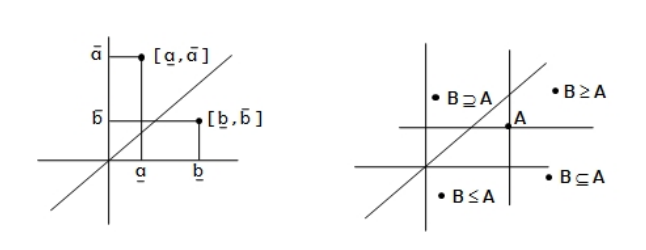
\includegraphics[scale=0.5]{images/florez11.png}
\caption{La primera imagen nos muestra la representación de los intervalos modales y la segunda las inclusiones y las desigualdades.}
\end{figure}

Las operaciones{ \em meet} y{ \em join} en $I^*(\mathbb{R})$ para una familia acodata de intervalos modales $A(I) := \{ A(i) = [a_1(i),a_2(i)] \in I^*(\mathbb{R}) : i \in I \}$, donde $I$ es el el dominio de índices, se definen por:

\begin{equation}
\wedge(i,I) A(i) = A \in I^*(\mathbb{R}) \text{ es  tal que } \forall (i,I) X \subset A(i) \iff X \subset A
\nonumber
\end{equation}
\begin{equation}
\vee(i,I) A(i) = B \in I^*(\mathbb{R}) \text{ es  tal que } \forall (i,I) X \supset A(i) \iff X \supset B
\nonumber
\end{equation}

anotado como $(A \wedge B)$ y $(A \vee B)$ para el caso correspondiente. El resultado, visto como función de los límites de los intervales, es:

\begin{equation}
\bigwedge_{i \in I} A(i) = [\max_{i \in I} a_1(i), \min_{i \in I} a_2(i)]
\nonumber
\end{equation}
\begin{equation}
\bigvee_{i \in I} A(i) = [\min_{i \in I} a_1(i), \max_{i \in I} a_2(i)]
\nonumber
\end{equation}

Con estas operaciones el conjunto de intervalos modales es un retículo para la $\subset$-relación, mientras que los intervalos clásicos no lo son, por tanto, estamos completando el conjunto de los intervalos clásicos.
\par Ambos operadores son insotónicos. i.e.,  si $A_i \subset B_i$ para cada $i \in I$, entonces:

\begin{equation}
\bigwedge_{i \in I} A_i \subset \bigwedge_{i \in I} B_i
\nonumber
\end{equation}

\begin{equation}
\bigvee_{i \in I} A_i \subset \bigvee_{i \in I} B_i
\nonumber
\end{equation}

En el conjunto de los números conocémos que hay dos relaciones $\leq$ y $\geq$ y las extensiones de estas relaciones a los intervalos se definen por:

\begin{equation}
[x_1,x_2] \leq [y_1,y_2] \iff x_i \leq y_i \hspace{0.5cm} i = 1,2
\nonumber
\end{equation}

Lo que nos conducea los operadores $\min$ y $\max$ para una familia acotada de intervalos modales $A(I) := \{ A(i) \in I^*(\mathbb{R}) : i \in I \}$ como:

\begin{equation}
\min_{i \in I} A(i) = A \in I^*(\mathbb{R}) \text{ es  tal que } \forall (i,I) X \leq A(i) \iff X \leq A
\nonumber
\end{equation}
\begin{equation}
\max_{i \in I} A(i) = B \in I^*(\mathbb{R}) \text{ es  tal que } \forall (i,I) X \geq A(i) \iff X \geq B
\nonumber
\end{equation}

Computacionalmente expresado:

\begin{equation}
\min_{i \in I} A(i) = [\min_{i \in I} a_1(i), \min_{i \in I} a_2(i)]
\nonumber
\end{equation}

\begin{equation}
\max_{i \in I} A(i) = [\max_{i \in I} a_1(i), \max_{i \in I} a_2(i)]
\nonumber
\end{equation}

El conjunto de los intervalos modales es, por tanto, un retículo bajo la $\leq$-relación. La siguiente figura nos muestra la representación geométrica de los operadores que hemos definido para dos intervalos:

\begin{figure}[h]
\centering
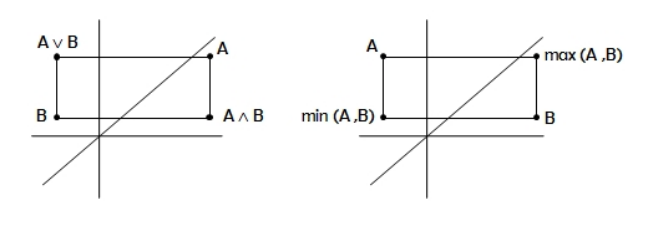
\includegraphics[scale=0.5]{images/florez12.png}
\end{figure}

\subsection{Extensiones semánticas}

En la teoría clásica de Análisis de Intervalos una extensión de una función de $\mathbb{R}^n$ a $\mathbb{R}$ dada por $z = f(x_1, \dotso, x_n)$ es el intervalo de extensión unida $R_f$ de $f$. Para el intervalo $X' = (X_1',\dotso, X_n') \in I(\mathbb{R}^n)$ se define el rango de $f$-valores en $X'$ como:

\begin{equation}
R_f(X_1',\dotso, X_n') := \{ f(x_1, \dotso, x_n) : x_i \in X_i' \ \forall i \in \{1, \dotso, n \} \} =
\nonumber
\end{equation}
\begin{equation}
= [\min \{ f(x_1, \dotso, x_n) : x_i \in X_i' \ \forall i \in \{1, \dotso, n \} \}, \max \{ f(x_1, \dotso, x_n) : x_i \in X_i' \ \forall i \in \{1, \dotso, n \} \}]
\nonumber
\end{equation}

Para obtener la estimación para la extensión unida, las extensiones racionales del intervalo teórico $fR(X_1', \dotso, X_n')$se definen como su correspondiente función real-racional $f(x_1, \dotso, x_n)$ reemplazando:

\begin{enumerate}
\item Los argumentos numéricos $x_i$ por sus argumentos de intervalos $X_i'$.
\item Los operadores aritméticos{ \em reales} $\omega$ por su correspondiene operación entre intervalos la cual, en los casos más comunes de computaciones truncadas de cualquier aritmética tiene que dirigirse al esterior $\omega^R$ debido a la inclusión:

$$X' \omega Y' \subset X' \omega^R Y' := Out(X' \omega Y')$$

Donde $Out$ representa el redondeo exterior del intervalo $X' \omega Y'$.
\end{enumerate}

Las funciones de intervalos raconales tienen la propiedad, fundamental para todo el cuerpo de Análisis de Intervalos, de ser inclusiva, esto es, para un conjunto de intervalos cumpliendo $X_1' \subset Y_1', \dotso, X_n' \subset Y_n'$ la siguiente relación se cumple, suponiendo que no ocurre  ninguna división entre un intervalo que contenga al cero.

\begin{equation}
f R(X_1', \dotso, X_n') \subset f R(Y_1', \dotso, Y_n')
\nonumber
\end{equation}

La relación entre ambas extensiones es:

\begin{equation}
R_f(X_1', \dotso, X_n') \subset f R(X_1', \dotso, X_n')
\nonumber
\end{equation}

Donde $f R$ es computable a parir de los límites de los intervalos $X_1', \dotso, X_n'$ y normalmente representan una sobrestimación de $R_f(X_1', \dotso, X_n')$.
\par En el Análisis de Intervalos Modales, un rol similar al de $R_f$ se ve cubierto de forma semántica por las funciones * y **, denotadas por $f^*$ y $f^{**}$ (funciones estrella y doble estrella) y definidas por:

\begin{equation}
f^*(X) := \bigvee_{x_p \in X_p'} \bigwedge_{x_i \in X_i'} [f(x_p,x_i),f(x_p,x_i)] = \left[ \min_{x_p \in X_p'} \max_{x_i \in X_i'} f(x_p,x_i), \max_{x_p \in X_p'} \min_{x_i \in X_i'} f(x_p,x_i) \right]
\nonumber
\end{equation}

\begin{equation}
f^{**}(X) := \bigwedge_{x_i \in X_i'} \bigvee_{x_p \in X_p'} [f(x_p,x_i),f(x_p,x_i)] = \left[ \max_{x_p \in X_p'} \min_{x_i \in X_i'} f(x_p,x_i), \min_{x_p \in X_p'} \max_{x_i \in X_i'} f(x_p,x_i) \right]
\nonumber
\end{equation}

Las cuales tienen, por supuesto, la propiedad de inclusión $f^*(X) \subset f^{**}(X)$. Además:

\begin{equation}
X \subset Y \Rightarrow f^*(X) \subset f^*(Y) \ \text{ y } \ f^{**}(X) \subset f^{**}(Y)
\nonumber
\end{equation}

En algunos casos puede ocurrir que $f^* \equiv f^{**}$.
\par Los próximos teoremas nos dan una interpretación lógica de las extensiones semánticas.

\begin{theorem}
nrwvprnpvngrw
\end{theorem}

\subsection{Interpretabilidad y optimización}

\section{Conclusiones}

En este capítulo hemos definido e introducido las diferentes propiedades del Análisis de Intervalos. Como hemos explicado, la Aritmética de Intervalos se puede aplicar a diversos campos de investigación para solucionar los problemas de redondeo. Por supuesto las gráficas por ordenador no iban a ser una excepción.
\par También hay una visión del Análisis de Intervalos Modales, que completa la definición clásica de Análisis de Intervalos mediante aplicación de los cuantificadores a la definición de intervalo. La teoría de Intervalos Modales nos da los intervalos impropios que en la teoría clásica carece de sentido y, en la mayoría de casos, la transformación lleva tal intervalo impropio en uno propio sin explicación lógica. El Análisis de Intervalos Modales nos concede una explicación para tales casos por medipo de las aplicaciones de los teoremas incluidos en este capítulo.
\par Los teoremas desarrollados son la base para la teoría de Intervalos Modales y, además, nos ayudarán a mejorar el Ray Tracing, o trazado, de superficies implícitas.